\chapter{Krav}
\label{chp:Krav}
Med udgangspunkt i afgrænsningen for projektet er der blevet opstillet en række krav for WinePrep. De funktionelle krav er beskrevet ved tre usecases, 
hvoraf de to mest betydende for WinePrep's værdi vil blive beskrevet nøjere i dette kapitel. Før disse beskrives er det dog påliggende at få sat nogle rammer på WinePrep i form af systemets 
grænseflader til dettes aktører. I figur \ref{fig:UCD_WP} ses de vigtigste usecases for WinePrep samt aktører.

\begin{figure}[H]
	\centerline{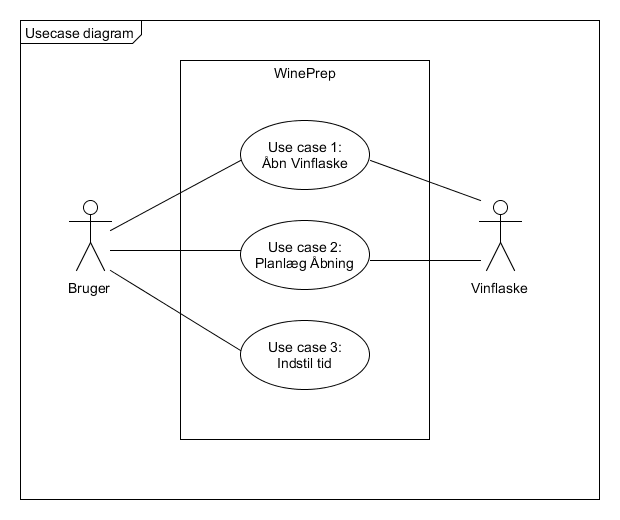
\includegraphics[scale=0.5]{Usecasediagram}}
	\caption{Usecase-diagram for WinePrep}
	\label{fig:UCD_WP}
\end{figure}

\section{Aktører}
Som set i figur \ref{fig:UCD_WP} er der to aktører for dette system: brugeren af WinePrep; og den givne vinflaske, der skal åbnes.

\subsection{Bruger}
Brugeren af WinePrep er den primære aktør. Denne indsætter en vinflaske i WinePrep og interagerer med systemet via dettes brugergrænseflade, 
hvormed brugeren kan benytte sig af produktets funktioner.

\subsection{Vinflaske}
Vinflasken indgår som en passiv aktør i systemet, der inspiceres og åbnes af WinePrep. Denne skal være af en bestemt type og ved indsættelse i WinePrep være i 
en bestemt tilstand. Mere om dette findes beskrevet i bilaget\footnote{Se Mål for kompatibel vinflaske}.

\section{Usecases}
De to vigtigste usecases vil her blive beskrevet overordnet. Mere information om disse og den tredje usecase kan findes i bilaget\footnote{Se kapitel 2.2 side 6 i Dokumentation}.

\subsection{Åbn vinflaske}
Brugeren skal efter at have indsat en vinflaske i WinePrep vælge funktionen "Åbn nu" på brugergrænsefladen. Systemet skal da foretage målinger af den indsatte 
vinflaske for at bekræfte, at denne er af en type, der er kompatibel med systemet. Herefter skal systemet åbne vinflasken og informere brugeren om dette. 
Løbende under processen vil der blive taget hånd om fejlscenarier, hvor brugeren via brugergrænsefladen vil blive informeret om, at vinflasken ikke er indsat korrekt 
eller er af en ukompatibel type, hvis denne ikke godkendes af systemet\footnote{Se kapitel 2.2 nederst på side 6 i Dokumentation}.

\subsection{Planlæg åbning}
Brugeren skal på brugergrænsefladen vælge funktionen "Planlæg åbning" og herefter på en menu vælge et tidspunkt, hvor 
vinflasken ønskes åbnet. Systemet venter da til det indtastede tidspunkt, hvor brugeren 
forinden skal have indsat vinflasken i WinePrep. Derefter påbegyndes proceduren beskrevet i "Åbn Vinflaske" ovenfor. Brugergrænsefladen vil herefter vise det 
tidspunkt, hvor vinen vil være drikkeklar\footnote{Se Ordliste}. Kan det ønskede tidspunkt, hvor vinen skal være drikkeklar, ikke forenes med iltningstidspunktet, annulleres processen, hvorefter brugeren vil blive tilbudt muligheden for at få vinflasken åbnet før det planlagte
åbningstidspunkt.

\section{Ikke-funktionelle krav}
- WinePrep skal have en brugergrænseflade, som skal indeholde knapper med billeder på, der illustrerer hver knaps funktion\footnote{Se GUI\_med\_billeder i bilag}. \\
- Disse knapper skal ligeledes have et flademål, som gør det muligt for brugeren at kunne trykke på disse med sin finger uden at ramme en naboknap. \\
- WinePrep skal kunne behandle brugerinput indenfor et fastsat tidsinterval og løbende holde brugeren opdateret om vinflaskens status. \\
- Vinflasken skal være af en på forhånd bestemt type\footnote{Se Mål for kompatibel vinflaske}. \\
- WinePrep skal kunne detektere vinflaskens centrum med en maksimal afvigelse på 1mm for at undgå, at vinflaskens prop knækker ifm. åbningen. \\
- Skulle der opstå et behov for reparation eller vedligeholdelse af systemet, skal en ekspert i WinePrep's interne konstruktion kontaktes. \\
\\
For yderligere informationer se bilag for ikke-funktionelle krav.